\documentclass[a4paper]{article}
\usepackage[english]{babel}
\usepackage[utf8]{inputenc}
\usepackage{textcomp}
\usepackage{amsmath}
\usepackage{gensymb}
\usepackage{physics}
\usepackage{graphicx}
\usepackage[colorinlistoftodos]{todonotes}
\usepackage{xcolor}
\usepackage{array}
\usepackage{tabularx}
\usepackage{tikz}
\usepackage{framed}
\usepackage{xfrac}
\usepackage[most]{tcolorbox}
\usepackage{fix-cm}
\usepackage[margin=0.5in]{geometry}
\usetikzlibrary{quotes,angles}
\usetikzlibrary{decorations.pathreplacing}
\usetikzlibrary{calc}

\let\phi\varphi
\let\bf\textbf
\colorlet{shadecolor}{orange!15}
\def\centerarc[#1](#2)(#3:#4:#5){\draw[#1] ($(#2)+({#5*cos(#3)},{#5*sin(#3)})$) arc (#3:#4:#5)}

\date{}
\author{}
\title{Week 10 Lecture Notes}

\begin{document}
\maketitle
\section{7/15 Lecture}
\bf{Torque $\boldsymbol{\vec{\tau}}$}
\begin{itemize}
    \item Analogous to force but for rotation
    \item Accelerates rotational motion
    \item Has units of Nm
\end{itemize}
\begin{align*}
    \sum \vec{F}_{net} &= m\vec{a}\\
    \vec{\tau} &= I\vec{\alpha} 
\end{align*}
If there is some net force then there must be some acceleration. $\sum F_{net} \neq 0$
\begin{align*}
    \tau = \vec{r} \times \vec{F} = |r||F|\sin(\phi)
\end{align*}
\begin{align*}
    \vec{A} \times \vec{B} = \vec{C}
\end{align*}

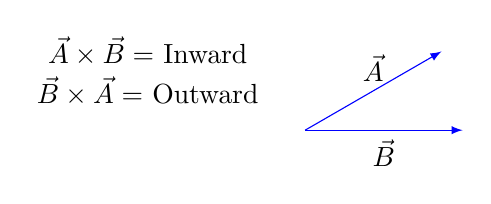
\begin{tikzpicture}[scale= 2]
    \draw[->,draw=blue,-latex] (0,0)--node[below]{$\vec{B}$} (1,0);
    \draw[->,draw=blue,-latex] (0,0)--node[above]{$\vec{A}$} ({cos(30)},{sin(30)});
    \node at (-1,0.5){$\vec{A} \times \vec{B} =$ Inward};
    \node at (-1,0.25){$\vec{B} \times \vec{A} =$ Outward};
\end{tikzpicture}
\begin{align*}
    \vec{A} \times \vec{B} = |\vec{A}||\vec{B}|\sin(\theta)\hat{n}
\end{align*}
Use the right hand rule to determine which direction\\
Anticommutative property: $\vec{A} \times \vec{B} = -\vec{B} \times \vec{A}$\\
The cross product between two parallel vectors is zero

\begin{align*}
    \vec{A} \cdot \vec{B} = |\vec{A}||\vec{B}_{\parallel}| = |\vec{A}_{\parallel}||\vec{B}|\\
    |\vec{A} \times \vec{B}| = |\vec{A}||\vec{B}_{\perp}|
\end{align*}
Comparison of Force and Torque
\begin{align*}
    \vec{F}_{tot} = m\vec{a} = \sum\vec{F}_i\\
    \vec{\tau} = I\vec{\alpha} = \sum\vec{r}_i \times \vec{F}_i
\end{align*}

\begin{shaded}
    \underline{\bf{Example:} Fly Fishing Event}
    \vspace{2mm}\\
    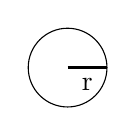
\begin{tikzpicture}
        \draw (0,0) circle (0.5);
        \draw[line width=1pt] (0,0)--node[below]{r}(0.5,0);
    \end{tikzpicture}
    \begin{align*}
        -I_{cm} = \frac{1}{2}MR^2 &= \frac{1}{2}(0.1)(6\times 10^{-2}\text{ m})^2\\
        &= 1.8\times 10^{-4}\text{ kgm}^2\\
    \end{align*}
    \begin{align*}
        I_{cm} &= \frac{1}{2}mr^2\\
        I'_{cm} &= I_{cm} + mR^2\\
        &= \frac{1}{2}mr^2 + mR^2 = 7.3 \times 10^{-5}\text{ kgm}^2 \\
        I_{reel} &= I_{cm} + I'_{cm} = 2.5\times 10^{-4}\text{ kgm}^2
    \end{align*}
    If you apply a force of 200 N tangent to the reel, what is the direction and magnitude of $\vec{\alpha}$:
    \begin{align*}
        \tau = R \times F = |R||F|\sin(90\degree) = I\vec{\alpha}\\
        6\times 10^{-2} \times (200\text{ N}) = 12\text{ Nm}\\
        \alpha = \frac{RFsin(\theta)}{I} = \frac{12}{2.5 \times 10^{-4}} = 4.8 \times 10^{4} rad\;s^{-2}
    \end{align*}
\end{shaded}

\end{document}